
\section{Getting Started with LaTeX}

\begin{frame}{What is LaTeX?}
    \begin{columns}
        \begin{column}{0.6\textwidth}
            \begin{itemize}
                \item A document preparation system using markup language
                \item Pronounced "Lay-tech" or "Lah-tech"
                \item Created by Leslie Lamport (based on TeX by Donald Knuth)
                \item Focuses on \alert{content} rather than \alert{appearance}
                \item Popular in academia, especially in mathematics
            \end{itemize}
        \end{column}
        
        \begin{column}{0.4\textwidth}
                
\includegraphics[width=0.7\linewidth]{figs/latex_logo}
        \end{column}
    \end{columns}
\end{frame}

\begin{frame}{Latex Creators}
    \begin{columns}
        \begin{column}{0.6\textwidth}
            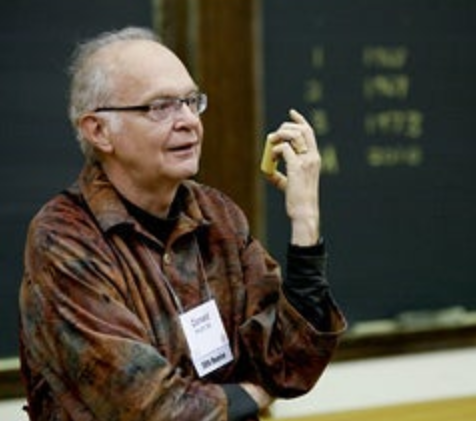
\includegraphics[width=0.7\linewidth]{figs/knuth}
        \end{column}
        
        \begin{column}{0.5\textwidth}
            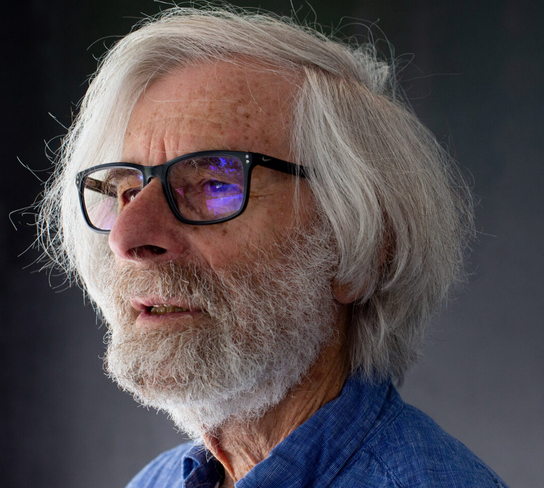
\includegraphics[width=0.9\linewidth]{figs/Lamport}
        \end{column}
    \end{columns}
\end{frame}


\begin{frame}{Latex vs. Word?}
	\begin{columns}
		\begin{column}{0.6\textwidth}
	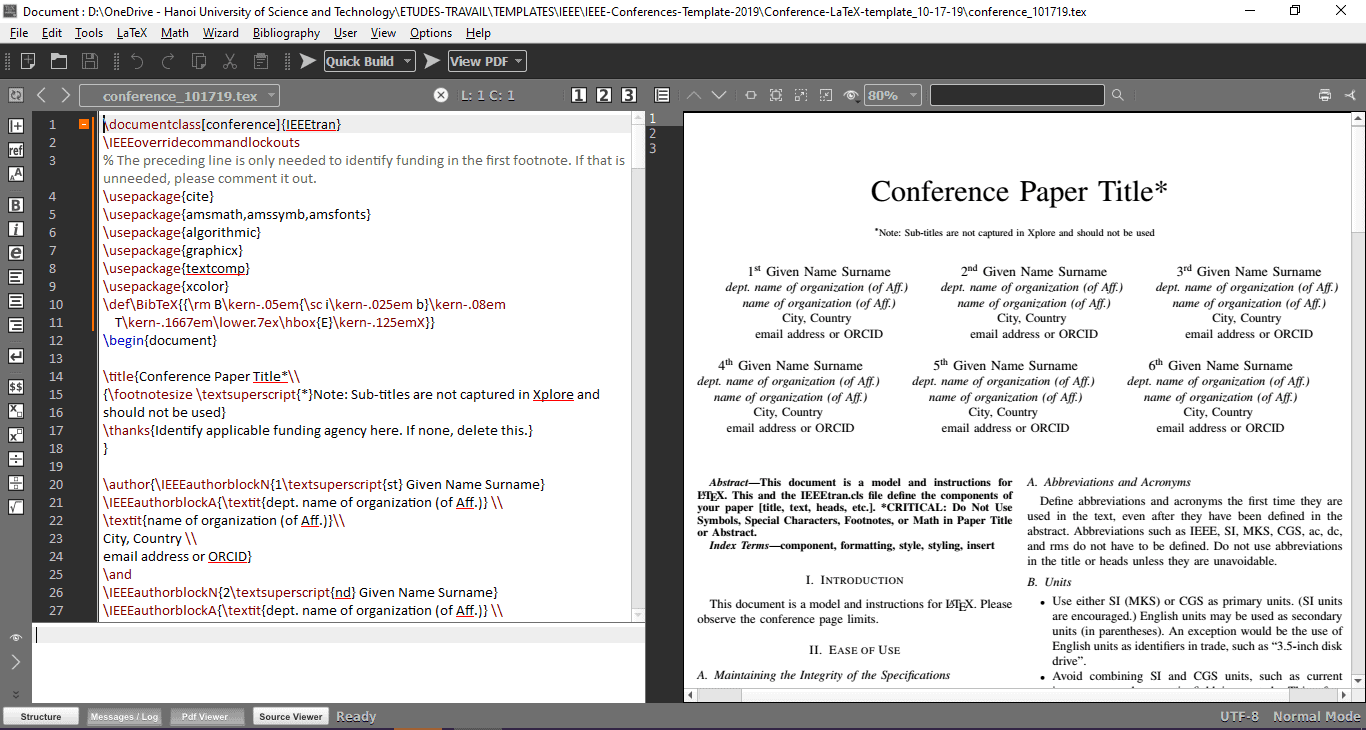
\includegraphics[width=0.9\linewidth]{figs/latex_code}
		\end{column}
		
		\begin{column}{0.4\textwidth}
	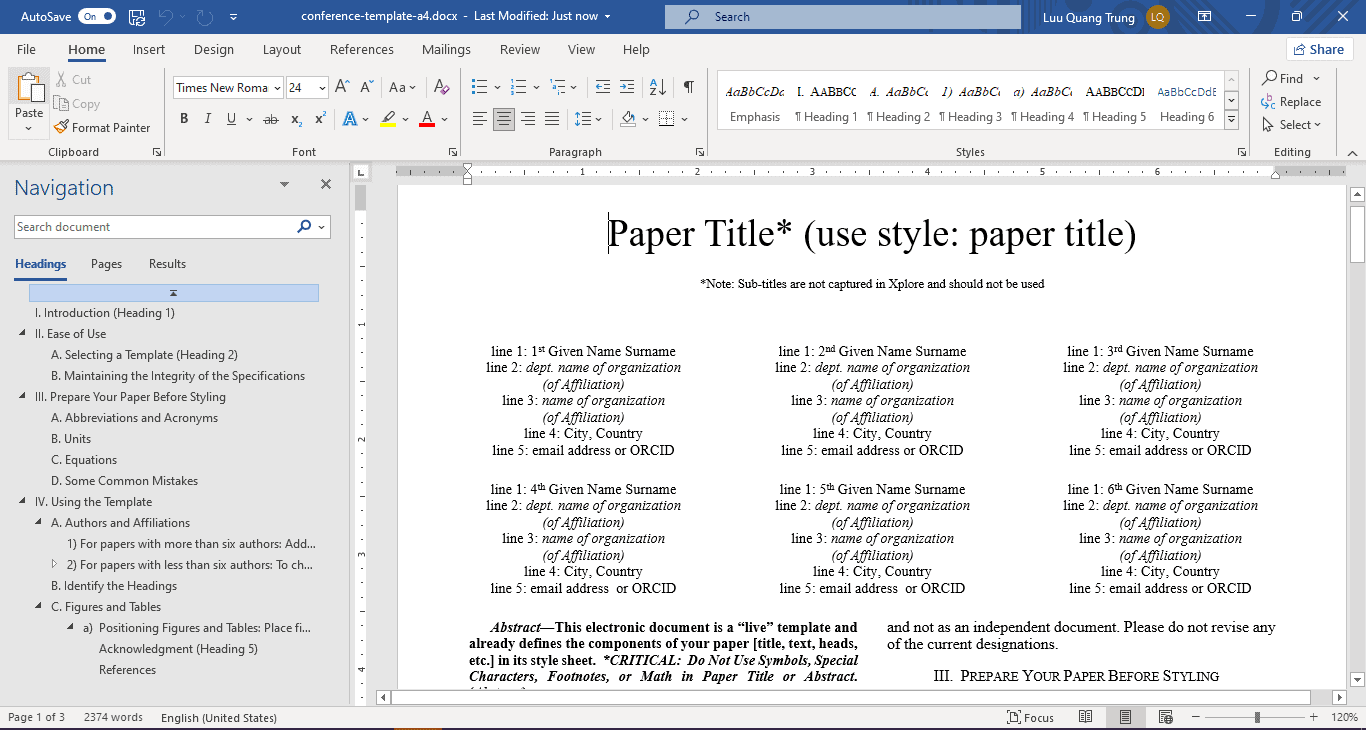
\includegraphics[width=1.0\linewidth]{figs/latex_code1}
		\end{column}
	\end{columns}
\end{frame}


\begin{frame}{Why Use LaTeX?}
    \begin{columns}
        \begin{column}{0.5\textwidth}
            \textbf{Strengths:}
            \begin{itemize}
                \item \alert{Professional typesetting} of mathematics
                \item Consistent formatting throughout documents
                \item Automatic numbering (equations, figures, etc.)
                \item Robust cross-referencing
                \item Bibliography management
                \item Scalable from short notes to books
                \item Stable and free
            \end{itemize}
        \end{column}
        
        \begin{column}{0.5\textwidth}
            %                \includegraphics[width=\textwidth]{example-image-b}
            \begin{center}
                Compare: Word vs. LaTeX output
            \end{center}
            
            \begin{alertblock}{LaTeX shines when:}
                \begin{itemize}
                    \item Documents contain complex mathematics
                    \item Consistency is crucial
                    \item Document will be revised multiple times
                \end{itemize}
            \end{alertblock}
        \end{column}
    \end{columns}
\end{frame}

\begin{frame}{LaTeX Workflow}
    \begin{enumerate}
        \item Write source code (.tex file)
        \item Compile the document
        \item View the output (PDF)
        \item Revise and repeat
    \end{enumerate}
    
    \begin{center}
        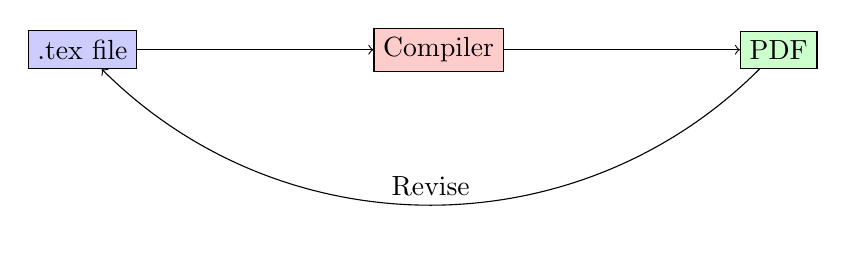
\begin{tikzpicture}[node distance=3cm, auto]
            \usetikzlibrary{positioning} % Add this line to load the positioning library
            \node (source) [rectangle, draw, fill=blue!20] {.tex file};
            \node (compile) [rectangle, draw, fill=red!20, right=of source] {Compiler};
            \node (output) [rectangle, draw, fill=green!20, right=of compile] {PDF};
            \draw[->] (source) -- (compile);
            \draw[->] (compile) -- (output);
            \draw[->] (output) to[bend left=45] node[above] {Revise} (source);
        \end{tikzpicture}
    \end{center}
    
    \begin{tip}
        Most LaTeX editors provide buttons for compile, view, and other common actions
    \end{tip}
\end{frame}

\begin{frame}[fragile]{Your First LaTeX Document}
    \begin{columns}
        \begin{column}{0.5\textwidth}
\begin{lstlisting}
\documentclass{article}

\begin{document}
    Hello, world!
    
    This is my first \LaTeX{} document.
\end{document}
\end{lstlisting}
        \end{column}
        
        \begin{column}{0.5\textwidth}
            \begin{itemize}
                \item Every document starts with \texttt{\textbackslash documentclass}
                \item The actual content goes between:
                \begin{itemize}
                    \item \texttt{\textbackslash begin\{document\}}
                    \item \texttt{\textbackslash end\{document\}}
                \end{itemize}
                \item Commands start with backslash \texttt{\textbackslash}
                \item Some commands take arguments in \{\}
            \end{itemize}
        \end{column}
    \end{columns}
    
    \begin{practice}
        Create this simple document in your editor and compile it
    \end{practice}
\end{frame}

\begin{frame}{Your First LaTeX Document: Complete Template}
	\begin{columns}
		\begin{column}{0.55\textwidth}
			\begin{lstlisting}[basicstyle=\small\ttfamily]
				% My first LaTeX document
				\documentclass{article}
				
				% ----- PREAMBLE -----
				% (Settings and packages go here)
				\usepackage{amsmath}  % For math
				\usepackage{graphicx} % For images
				\usepackage[margin=1in]{geometry} % Page layout
				
				% Document information
				\title{My First \LaTeX{} Document}
				\author{Your Name}
				\date{\today}
				
				% ----- DOCUMENT CONTENT -----
				\begin{document}
					
					\maketitle  % Creates title from info above
					
					\section{Introduction}
					Hello world! This is my first \LaTeX{} document.
					It supports mathematics like $E = mc^2$.
					
					\section{A List of Items}
					\begin{itemize}
						\item First item
						\item Second item
						\item Third item with math: $\alpha^2 + \beta^2$
					\end{itemize}
					
				\end{document}
			\end{lstlisting}
		\end{column}
		
		\begin{column}{0.45\textwidth}
			\begin{alertblock}{File structure explained}
				\begin{enumerate}
					\item \textbf{Preamble}: Everything before \verb|\begin{document}|
						\begin{itemize}
							\item Document class
							\item Packages
							\item Title information
						\end{itemize}
						\item \textbf{Body}: Everything between \verb|\begin{document}| and \verb|\end{document}|
						\begin{itemize}
							\item Actual content appears here
							\item Sections, text, math, etc.
						\end{itemize}
					\end{enumerate}
				\end{alertblock}
				
				\begin{tip}
					Save this as \texttt{firstdoc.tex} and compile it to see the result!
				\end{tip}
			\end{column}
		\end{columns}
	\end{frame}

\begin{frame}[fragile]{Document Classes}
    \begin{columns}
        \begin{column}{0.5\textwidth}
            \begin{lstlisting}
\documentclass[12pt,a4paper]{article}
\documentclass{report}
\documentclass{book}
\documentclass{letter}
\documentclass{beamer}
            \end{lstlisting}
        \end{column}
        
        \begin{column}{0.5\textwidth}
            \begin{itemize}
                \item \texttt{article}: Short documents, papers
                \item \texttt{report}: Longer reports with chapters
                \item \texttt{book}: Full books
                \item \texttt{letter}: Correspondence
                \item \texttt{beamer}: Presentations (like this one!)
            \end{itemize}
            
            \textbf{Options in square brackets:}
            \begin{itemize}
                \item Font size: \texttt{10pt}, \texttt{11pt}, \texttt{12pt}
                \item Paper size: \texttt{a4paper}, \texttt{letterpaper}
                \item Columns: \texttt{twocolumn}, \texttt{onecolumn}
                \item And many more...
            \end{itemize}
        \end{column}
    \end{columns}
\end{frame}

\begin{frame}{Comments and Useful Tips in \LaTeX}
	
	\begin{itemize}
		\item \textbf{Comments} in \LaTeX: use the \texttt{\%} symbol
		\begin{itemize}
			\item Example: \texttt{\% This is a comment, it will not appear in the output}
			\item Everything after \texttt{\%} on the same line is ignored.
		\end{itemize}
		\vspace{0.3cm}
		
		\item \textbf{Spacing}: multiple spaces and line breaks are treated as a single space.
%		\begin{itemize}
%			\item To force a new line, use \verb|\\|.
%			\item For more vertical space: \verb|\vspace{length}|.
%		\end{itemize}
		\vspace{0.3cm}
		
		\item \textbf{Special Characters}: some symbols must be escaped.
		\begin{itemize}
			\item Examples: \texttt{\$ \% \_ \{ \} \# \& \textbackslash}.
			\item To print them, use \texttt{\textbackslash} before the character, e.g., \texttt{\textbackslash\%}.
		\end{itemize}
		
		\vspace{0.3cm}
		\item \textbf{Good Practice}: use comments to document your source code.
		\begin{itemize}
			\item Helps collaborators and your future self.
			\item Example: \texttt{\% This section introduces the main theorem.}
		\end{itemize}
%		
	\end{itemize}
	
\end{frame}

\begin{frame}[fragile]{The Preamble and Packages}
    \begin{columns}
        \begin{column}{0.5\textwidth}
            \begin{lstlisting}
\documentclass{article}

% This is the preamble
\usepackage{amsmath}
\usepackage{amssymb}
\usepackage{graphicx}
\usepackage[margin=1in]{geometry}
\usepackage{hyperref}

\title{My Mathematics Document}
\author{Your Name}
\date{\today}

\begin{document}
    \maketitle
    % Document content here...
\end{document}
            \end{lstlisting}
        \end{column}
        
        \begin{column}{0.5\textwidth}
            \begin{itemize}
                \item The \alert{preamble} is everything between the document class and \texttt{\textbackslash begin\{document\}}
                \item \texttt{\textbackslash usepackage} adds functionality
                \item Common packages for mathematics:
                \begin{itemize}
                    \item \texttt{amsmath}: Enhanced math features
                    \item \texttt{amssymb}: Additional math symbols
                    \item \texttt{graphicx}: For including images
                    \item \texttt{geometry}: Page layout control
                    \item \texttt{hyperref}: PDF links and bookmarks
                \end{itemize}
            \end{itemize}
        \end{column}
    \end{columns}
    
    \begin{tip}
        Packages can have options in square brackets: \texttt{\textbackslash usepackage[options]\{package\}}
    \end{tip}
\end{frame}

\begin{frame}[fragile]{Document Structure}
    \begin{columns}
        \begin{column}{0.5\textwidth}
            \begin{lstlisting}
\documentclass{article}
\usepackage{amsmath}

\begin{document}
    \title{Introduction to Calculus}
    \author{Dr. Mathematics}
    \date{June 2025}
    \maketitle
    
    \section{Introduction}
    Calculus is fundamental to...
    
    \section{Derivatives}
    \subsection{Definition}
    The derivative is defined as...
    
    \subsection{Rules}
    Product rule, chain rule...
    
    \section{Conclusion}
\end{document}
            \end{lstlisting}
        \end{column}
        
        \begin{column}{0.5\textwidth}
            \textbf{Sectioning commands:}
            \begin{itemize}
                \item \texttt{\textbackslash section\{Title\}}
                \item \texttt{\textbackslash subsection\{Title\}}
                \item \texttt{\textbackslash subsubsection\{Title\}}
            \end{itemize}
            
            \textbf{For book/report classes:}
            \begin{itemize}
                \item \texttt{\textbackslash chapter\{Title\}} (highest level)
                \item \texttt{\textbackslash part\{Title\}} (even higher)
            \end{itemize}
            
            \textbf{Unnumbered versions:}
            \begin{itemize}
                \item \texttt{\textbackslash section*\{Title\}}
            \end{itemize}
        \end{column}
    \end{columns}
\end{frame}

\begin{frame}[fragile]{Basic Text Formatting}
    \begin{columns}
        \begin{column}{0.5\textwidth}
\begin{lstlisting}
% Font styles
Normal text
\textbf{Bold text}
\textit{Italic text}
\underline{Underlined text}
\texttt{Monospace text}

% Size changes
{\tiny Tiny text} 
{\small Small text}
{\large Large text} 
{\huge Huge text}

% Special characters
\& \% \$ \# \_ \{ \} \~{} \^{} 
\textbackslash

% New paragraph
First paragraph.

Second paragraph.
\end{lstlisting}
        \end{column}
        
        \begin{column}{0.5\textwidth}
            \textbf{Font styles:}
            \begin{itemize}
                \item Normal text
                \item \textbf{Bold text}
                \item \textit{Italic text}
                \item \underline{Underlined text}
                \item \texttt{Monospace text}
            \end{itemize}
            
            \textbf{Size changes:}
            {\tiny Tiny text} {\small Small text} Normal text {\large Large text} {\huge Huge text}
            
            \textbf{Special characters:}
            \& \% \$ \# \_ \{ \} \~{} \^{} \textbackslash
            
            \textbf{New paragraph:} Empty line (not indentation)
        \end{column}
    \end{columns}
\end{frame}

\begin{frame}[fragile]{Lists}
    \begin{columns}
        \begin{column}{0.5\textwidth}
\begin{lstlisting}
% Unordered list (bullet points)
\begin{itemize}
    \item First item
    \item Second item
    \begin{itemize}
        \item Nested item
        \item Another nested item
    \end{itemize}
    \item Third item
\end{itemize}

% Ordered list (numbered)
\begin{enumerate}
    \item First step
    \item Second step
    \begin{enumerate}
        \item Substep A
        \item Substep B
    \end{enumerate}
    \item Third step
\end{enumerate}
\end{lstlisting}
        \end{column}
        
        \begin{column}{0.5\textwidth}
            \textbf{Unordered list:}
            \begin{itemize}
                \item First item
                \item Second item
                \begin{itemize}
                    \item Nested item
                    \item Another nested item
                \end{itemize}
                \item Third item
            \end{itemize}
            
            \textbf{Ordered list:}
            \begin{enumerate}
                \item First step
                \item Second step
                \begin{enumerate}
                    \item Substep A
                    \item Substep B
                \end{enumerate}
                \item Third step
            \end{enumerate}
        \end{column}
    \end{columns}
\end{frame}

\begin{frame}[fragile]{Simple Tables}
    \begin{columns}
        \begin{column}{0.5\textwidth}
            \begin{lstlisting}
\begin{center}
    \begin{tabular}{|l|c|r|}
        \hline
        Left & Center & Right \\
        \hline
        1 & 2 & 3 \\
        4 & 5 & 6 \\
        \hline
    \end{tabular}
\end{center}

% Professional tables with booktabs
\begin{center}
    \begin{tabular}{lcr}
        \toprule
        Left & Center & Right \\
        \midrule
        1 & 2 & 3 \\
        4 & 5 & 6 \\
        \bottomrule
    \end{tabular}
\end{center}
            \end{lstlisting}
        \end{column}
        
        \begin{column}{0.5\textwidth}
            \begin{center}
                \begin{tabular}{|l|c|r|}
                    \hline
                    Left & Center & Right \\
                    \hline
                    1 & 2 & 3 \\
                    4 & 5 & 6 \\
                    \hline
                \end{tabular}
            \end{center}
            
            \textbf{With booktabs package (professional):}
            \begin{center}
                \begin{tabular}{lcr}
                    \toprule
                    Left & Center & Right \\
                    \midrule
                    1 & 2 & 3 \\
                    4 & 5 & 6 \\
                    \bottomrule
                \end{tabular}
            \end{center}
            
            \textbf{Column alignment:}
            \begin{itemize}
                \item \texttt{l} - left align
                \item \texttt{c} - center align
                \item \texttt{r} - right align
                \item \texttt{|} - vertical line
            \end{itemize}
        \end{column}
    \end{columns}
\end{frame}

\begin{frame}{Exercise 1: Basic Document Structure}
    \begin{practice}
        \textbf{Create a 1-page document with:}
        \begin{enumerate}
            \item Title, author, date
            \item Section and subsection headings
            \item A paragraph with bold and italic text
            \item A numbered list and a bullet-point list
            \item A simple table
        \end{enumerate}
    \end{practice}
    
    \begin{tip}
        \begin{itemize}
            \item Start with the basic document structure
            \item Add elements one by one
            \item Compile after adding each element to catch errors quickly
        \end{itemize}
    \end{tip}
\end{frame}
